\documentclass[]{article}
\usepackage{caption,subcaption,graphicx,float,url,amsmath,amssymb,amsthm,tocloft,cancel,thmtools,gensymb,braket}
\usepackage[toc,nonumberlist]{glossaries}
\usepackage{glossaries-extra}
\newcommand\numberthis{\addtocounter{equation}{1}\tag{\theequation}}

\newtheorem{thm}{Theorem}
\newtheorem{defn}[thm]{Definition}
\newtheorem{cor}[thm]{Corollary}
\newtheorem{lemma}[thm]{Lemma}
\graphicspath{{figs/}}
\widowpenalty10000
\clubpenalty10000
\setcounter{tocdepth}{2}

%opening
\title{Theoretical Minimum\\Particle Physics 2\\Standard Model}
\author{Simon Crase(compiler)}

\begin{document}

\maketitle

\begin{abstract}
These are my notes for the \emph{New Revolutions in Particle Physics 2} lectures from Leonard Susskind's \emph{Theoretical Minimum} series\cite{susskind2009standard}.
\end{abstract}

\tableofcontents
\listoffigures

\section{Particles fields and forces}

There is a triangle of concepts:
\begin{itemize}
	\item particles (quanta of fundamental fields)\footnote{We are going to have to think very hard about what is an elementary particles and what is composite always be frustrated, always find some slipper region why your definition did not work.}
	\item Fields
	\item Forces
\end{itemize}

\begin{figure}[H]
	\begin{center}
		\caption{Triangle of concepts: particles, fields, and forces}
		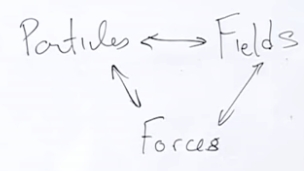
\includegraphics[width=0.5\textwidth]{ParticlesFieldsForces}
	\end{center}
\end{figure}

Consider two electric charges

\begin{align*}
E=&\int (e_1 \vec{E_1})^2 dV\\
E=&\int (e_2 \vec{E_2})^2 dV\\
E=&\int (e_1\vec{E_1}+e_2 \vec{E_2})^2 dV\\
=&\int \underbrace{(e_1\vec{E_1})^2}_\text{self energy}+ \underbrace{(e_2\vec{E_2})^2}_\text{self energy} + \underbrace{2e_1e_2\vec{E_1}.\vec{E_2}}_\text{interesting term}
\end{align*}

The first two terms represent self energy, which is includes in mass; the last term is proportional to the charges.
\begin{itemize}
	\item  If they are so far away that $\vec{E_1}$ is negligible near second charge there will be no perceptible effect.
	\item If the particles are close we will get a contribution from $\vec{E_1}.\vec{E_2}$. This turns out to be the Coulumb force. 
\end{itemize}

The force comes from the distortion of the field: this is a \emph{purely field view of forces}. If fields give rise to forces, and particles are quanta of fields, there must be a way to think of forces coming from particles.

Where do molecular forces come from? There are several mechanisms: we will focus on one. Imagine two protons and a single electron. Electron hops because of tennelling. \footnote{Don't watch tunnelling! Like any QM effect, watching ruins it.}

\begin{figure}[H]
	\caption[Molecular forces: two protons and a single electron]{Two protons and a single electron. Classically electron can't swap between Figures \ref{fig:2proton1Electrona} and \ref{fig:2proton1Electronb}, but QM allows it to tunnel.}
	\begin{subfigure}{0.45\textwidth}
		\caption{Right hand protons is a long way from Left: Schr\"odinger wave function for electron near left hand.} 
		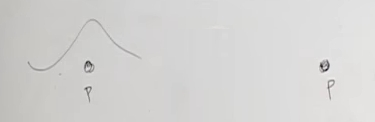
\includegraphics[width=0.9\textwidth]{2proton1Electrona}\label{fig:2proton1Electrona}
	\end{subfigure}
	\begin{subfigure}{0.45\textwidth}
		\caption{Protons closer together: Figure \ref{fig:2proton1Electrona} still possible, but so is this--same energy.}
		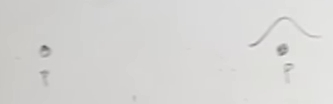
\includegraphics[width=0.9\textwidth]{2proton1Electronb}\label{fig:2proton1Electronb}
	\end{subfigure}
	\begin{subfigure}{0.45\textwidth}
		\caption{Effect of tunnelling}
		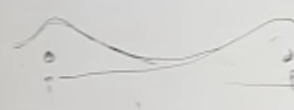
\includegraphics[width=0.9\textwidth]{2proton1Electronab}\label{fig:2proton1Electronab}
	\end{subfigure}
	\begin{subfigure}{0.45\textwidth}
		\caption{Energy as a function of distance between protons. Gradient in energy tries to move protons together, but Coulomb force tries to separate them. Nett effect is a covalent bond.}
		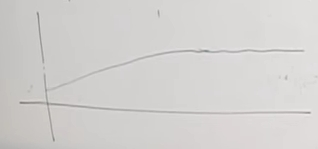
\includegraphics[width=0.9\textwidth]{2proton1ElectronEnergy}\label{fig:2proton1ElectronEnergy}
	\end{subfigure}
	\begin{subfigure}{0.45\textwidth}
		\caption{Electron exchange between protons. This lowers energy, leading to attraction.}
		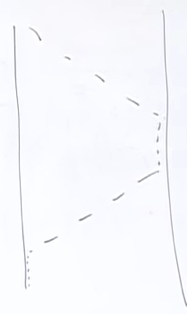
\includegraphics[width=0.9\textwidth]{2proton1ElectronHopping}\label{fig:2proton1ElectronHopping}
	\end{subfigure}
\end{figure}

Key idea: adding wave functions leads to a lower energy state. Energy lowered by alternating between states.

Add 2nd electron, then total charge is zero, giving nett attraction. 

\begin{itemize}
	\item So classically, add 2nd charge, lower energy (creates force) by distorting wave function.
	\item In QM, possibility of swapping between states lowers energy.
\end{itemize}
Can we think of Coulumb force in QM terms?

\url{https://youtu.be/Igl8hE3Eac0?t=1769}

\subsection{Renormalization}

\subsection{The equivalence of particles, fields, and forces}

\subsection{The particle zoo}

\section{Quantum chromodynamics}



\section{Group theory – part 1}



\section{Group theory – part 2}



\section{Gauge fields and symmetry}



\section{The weak interaction}



\section{Spontaneous symmetry breaking and Goldstone bosons}



\section{The Higgs field}






\section{The Higgs field and fermions}



\section{Renormalization and the running of coupling constants}




\bibliographystyle{unsrt}
\addcontentsline{toc}{section}{Bibliography}
\bibliography{tm}


\end{document}
